% PerfectMatchLFP26 staff manual. Compile twice: pdflatex manual.tex
\documentclass[11pt,a4paper]{article}
\usepackage[T1]{fontenc}
\usepackage[utf8]{inputenc}
\usepackage{lmodern}
\renewcommand{\familydefault}{\sfdefault}
\usepackage[margin=2cm,top=2.3cm,bottom=2.3cm]{geometry}
\usepackage{microtype}
\usepackage{graphicx}
\usepackage{xcolor}
\usepackage{tikz}
\usepackage{tabularx,booktabs,array}
\usepackage{enumitem}
\usepackage{fancyhdr}
\usepackage{titlesec}
\usepackage{amssymb}
\usepackage[most]{tcolorbox}
\usepackage[font=small,labelfont=bf,skip=4pt]{caption}
\usepackage[hidelinks]{hyperref}

\definecolor{accent}{HTML}{1D6B55}
\definecolor{accentsoft}{HTML}{E5F1EC}
\definecolor{ink2}{HTML}{52514E}
\definecolor{line}{HTML}{C3C2B7}
\definecolor{warnsoft}{HTML}{FFF5DC}
\definecolor{warnink}{HTML}{6B4A00}
\definecolor{gOne}{HTML}{C4372F}
\definecolor{gTwo}{HTML}{F0A090}
\definecolor{gThree}{HTML}{DCDAD2}
\definecolor{gFour}{HTML}{86B6EF}
\definecolor{gFive}{HTML}{1C5CAB}

\setlist{itemsep=2pt,topsep=4pt}
\setlength{\parindent}{0pt}
\setlength{\parskip}{5pt}
\titleformat{\section}{\Large\bfseries\color{accent}}{\thesection}{0.6em}{}
\titleformat{\subsection}{\large\bfseries}{\thesubsection}{0.6em}{}
\titlespacing*{\section}{0pt}{14pt}{6pt}
\titlespacing*{\subsection}{0pt}{10pt}{4pt}
\pagestyle{fancy}
\fancyhf{}
\renewcommand{\headrulewidth}{0.4pt}
\fancyhead[L]{\small\color{accent}PerfectMatchLFP26}
\fancyhead[R]{\small Staff manual}
\fancyfoot[L]{\small Local Friendship Programme 2026 \textbullet{} October 2026}
\fancyfoot[R]{\small\thepage}

\newcommand{\ui}[1]{\textbf{#1}}
\newcommand{\grade}[1]{{\setlength{\fboxsep}{2.2pt}\setlength{\fboxrule}{0.5pt}%
  \ifcase#1\or\colorbox{gOne}{\textcolor{white}{\textbf{\,1\,}}}%
  \or\colorbox{gTwo}{\textbf{\,2\,}}%
  \or\fcolorbox{line}{gThree}{\textbf{\,3\,}}%
  \or\colorbox{gFour}{\textbf{\,4\,}}%
  \or\colorbox{gFive}{\textcolor{white}{\textbf{\,5\,}}}\fi}}
\newcommand{\flagicon}{\tikz[baseline=-0.1ex]{\draw[line width=0.7pt,warnink] (0,-0.05) -- (0,0.3);
  \fill[warnink] (0,0.3) -- (0.2,0.24) -- (0,0.16) -- cycle;}}
\newcommand{\callout}[3]{\node[circle,fill=accent,text=white,font=\bfseries\footnotesize,
  inner sep=0pt,minimum size=5.2mm,draw=white,line width=0.8pt] at (#1,#2) {#3};}
\newcommand{\key}[1]{\tikz[baseline=-0.6ex]\node[circle,fill=accent,text=white,font=\bfseries\scriptsize,
  inner sep=0pt,minimum size=4.4mm]{#1};}
\newtcolorbox{tip}[1][Tip]{colback=accentsoft,colframe=accentsoft,coltitle=accent,fonttitle=\bfseries,
  title=#1,boxrule=0pt,arc=2mm,left=3mm,right=3mm,top=1mm,bottom=1mm,attach title to upper={\ }}
\newtcolorbox{caution}[1][Important]{colback=warnsoft,colframe=warnsoft,coltitle=warnink,fonttitle=\bfseries,
  title=#1,boxrule=0pt,arc=2mm,left=3mm,right=3mm,top=1mm,bottom=1mm,attach title to upper={\ }}
\newcommand{\shot}[2][\textwidth]{{\centering\setlength{\fboxsep}{0pt}\fcolorbox{line}{white}{\includegraphics[width=\dimexpr#1-1pt\relax]{#2}}\par}}

\begin{document}

{\color{accent}\rule{\textwidth}{1.2pt}}\par\vspace{2pt}
{\Huge\bfseries PerfectMatch\textcolor{accent}{LFP26}}\par\vspace{4pt}
{\Large Staff manual: suggesting international--local friend pairs}\par\vspace{2pt}
{\color{ink2}Local Friendship Programme 2026 \textbullet{} University of Jyväskylä}\par
{\color{accent}\rule{\textwidth}{1.2pt}}

\begin{tcolorbox}[colback=white,colframe=accent,boxrule=0.8pt,arc=2mm,left=4mm,right=4mm,
  title=In one minute,fonttitle=\bfseries,colbacktitle=accent]
PerfectMatchLFP26 reads the survey export and suggests one local friend for every international
student whenever the rules allow it. Each pair is graded like a school report, from
\grade{1}~insufficient to \grade{5}~perfect. You stay in control: change the weights or anyone's
must-have, compute again, compare, and save the result. Everything runs on your own computer.
\begin{enumerate}[leftmargin=*,label=\textbf{\arabic*.}]
  \item \ui{Load} the survey CSV.
  \item \ui{Set} the weights (or keep the defaults).
  \item \ui{Check} the must-haves, especially the ones marked in red.
  \item \ui{Compute} and read the results.
  \item \ui{Improve}: lock good pairs, forbid unsuitable ones, adjust must-haves, compute again.
  \item \ui{Save} result.csv, report.txt, settings.csv and must\_haves.csv.
\end{enumerate}
\end{tcolorbox}

\section{Start and stop}
\begin{enumerate}[leftmargin=*]
  \item Right-click \textbf{PerfectMatchLFP26-Windows.zip} and choose \ui{Extract All}.
  \item Open the extracted \textbf{PerfectMatchLFP26} folder and double-click \textbf{PerfectMatchLFP26.exe}.
        Keep the \texttt{\_internal} folder next to it. Nothing needs to be installed.
  \item Your web browser opens at \textbf{http://localhost:8766}. ``Localhost'' means your own computer;
        no internet connection is used.
  \item When you have finished and saved your files, click \ui{Close app} at the top right.
        Closing the browser tab alone does not stop the app.
\end{enumerate}
\begin{tip}[First time?]
Click \ui{Try fictional example} and follow this manual with it. The example has 20 internationals and
28 locals who do not exist. The screenshots in this manual show this example.
\end{tip}

\section{The screen at a glance}
The \textbf{left side} is where you work (the \emph{interact} phase). The \textbf{right side} shows the result of
each computation (the \emph{compute} phase). You switch between the two as often as you like.

The numbers and letters in Figure~\ref{fig:overview} are used throughout this manual.

\begin{figure}[t]
\centering
\begin{tikzpicture}
\node[anchor=south west,inner sep=0,draw=line] (img) at (0,0) {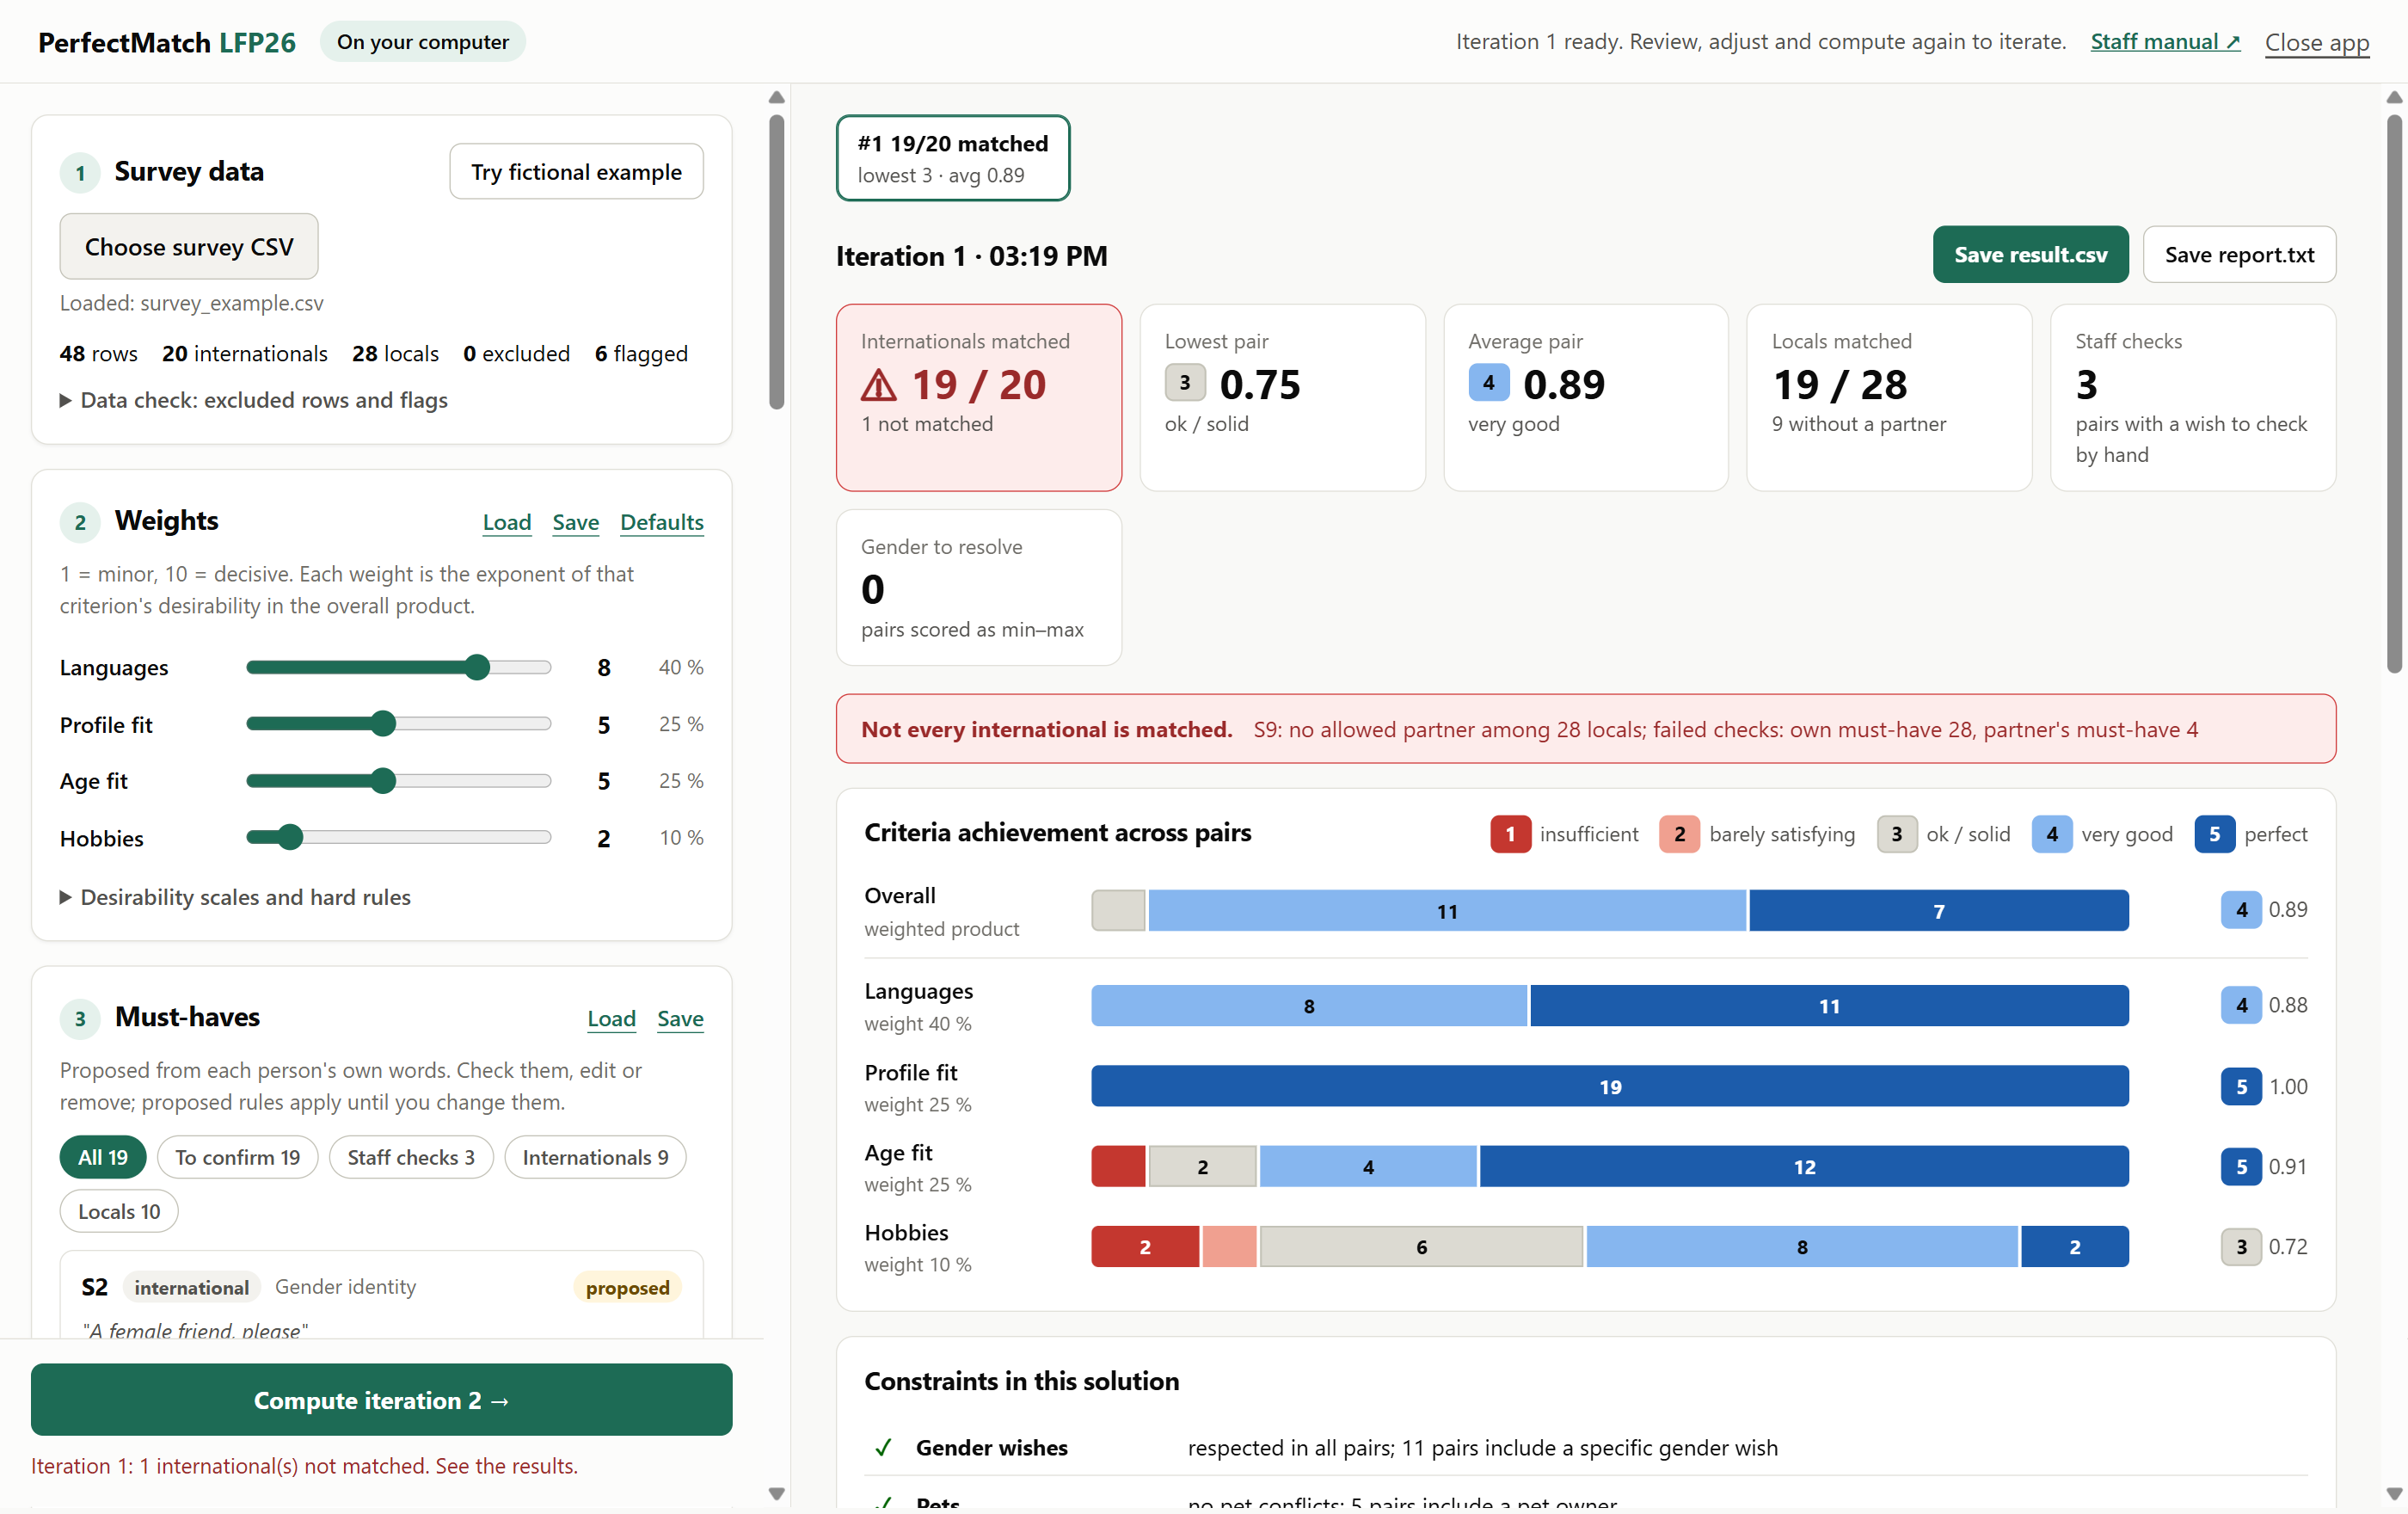
\includegraphics[width=\dimexpr\textwidth-1pt\relax]{manual/iteration1.png}};
\begin{scope}[x={(img.south east)},y={(img.north west)}]
  \callout{0.016}{0.92}{1}
  \callout{0.016}{0.69}{2}
  \callout{0.016}{0.36}{3}
  \callout{0.016}{0.075}{4}
  \callout{0.343}{0.925}{A}
  \callout{0.343}{0.80}{B}
  \callout{0.343}{0.535}{C}
  \callout{0.343}{0.478}{D}
  \callout{0.343}{0.115}{E}
  \callout{0.798}{0.852}{F}
\end{scope}
\end{tikzpicture}
\vspace{2pt}
{\small
\begin{tabularx}{\textwidth}{@{}lX@{\hspace{10pt}}lX@{}}
\key{1} & Survey data: load the CSV, see the data check & \key{A} & Iterations: one chip per computation \\
\key{2} & Weights: how much each criterion counts & \key{B} & Tiles: the most important numbers \\
\key{3} & Must-haves: each person's hard wish & \key{C} & Warning when an international is not matched \\
\key{4} & Compute the next iteration & \key{D} & Criteria achievement: grades of all pairs \\
 & & \key{E} & Constraints: which rules the solution respects \\
 & & \key{F} & Save result.csv and report.txt \\
\end{tabularx}}
\caption{The workspace after the first computation of the fictional example.}
\label{fig:overview}
\end{figure}

\section{Step by step}

\subsection*{Step 1 \textbullet{} Load the survey}
Export the survey results as \textbf{CSV} with \textbf{both heading rows} (the question row and the option row).
Do not edit the export by hand. Click \ui{Choose survey CSV} \key{1} and select the file. The app accepts
both ``CSV'' and ``CSV UTF-8'' from Excel.

The line under the button tells you how many rows were read, how many internationals and locals are
included, and how many rows were \emph{excluded} or \emph{flagged}. Open \ui{Data check} to see why.
\begin{itemize}[leftmargin=*]
  \item \textbf{Excluded} (left out of the matching): the ID is missing or appears twice, the status is not clearly
        ``local resident'' or ``international student'', a consent statement was not accepted, the row is damaged,
        or more than 2 of the 8 key answers are missing.
  \item \textbf{Flagged} (included, but please look): for example a blank own gender (``to be resolved''), pet answers
        that contradict each other, or a must-have without an explanation.
\end{itemize}

\subsection*{Step 2 \textbullet{} Set the weights}
\begin{minipage}[t]{0.47\textwidth}
\vspace{0pt}
\setlength{\fboxsep}{0pt}\fcolorbox{line}{white}{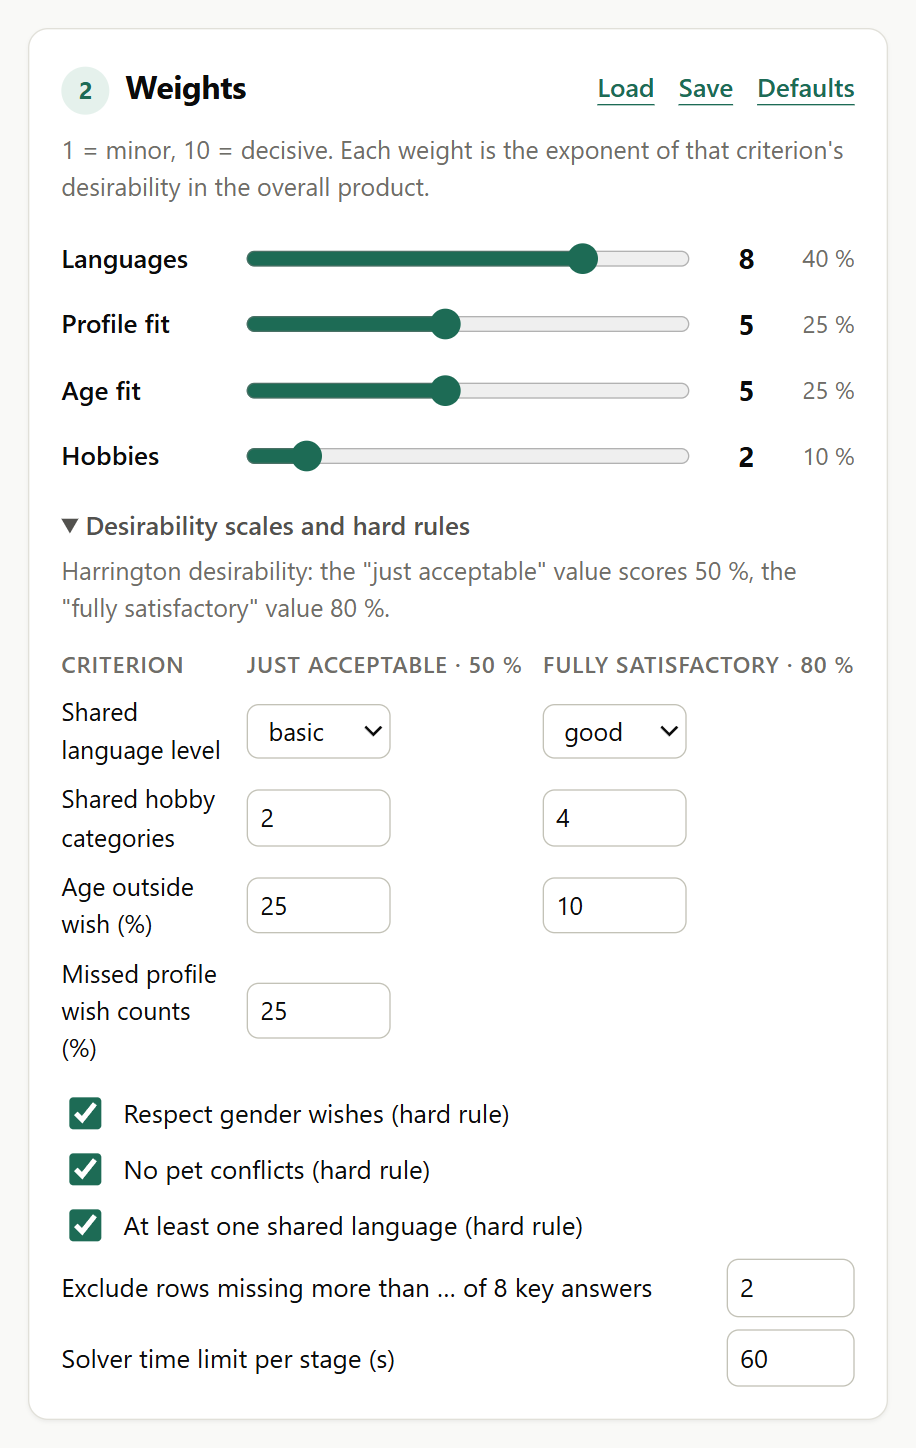
\includegraphics[width=\linewidth]{manual/weights.png}}
\end{minipage}\hfill
\begin{minipage}[t]{0.49\textwidth}
\vspace{0pt}
Four things decide how good a pair is. Move a slider from \textbf{1 (minor)} to \textbf{10 (decisive)}.
The percentage on the right shows each criterion's share; the defaults are 40/25/25/10\,\%.

\smallskip
{\small
\begin{tabularx}{\linewidth}{@{}>{\bfseries}lX@{}}
\toprule
Languages & the best language both speak, at the lower of the two levels \\
Profile fit & does each person fit what the other asked for (one person, couple, family, \ldots) \\
Age fit & is each person in the age range the other asked for \\
Hobbies & how many of the 13 hobby categories they share \\
\bottomrule
\end{tabularx}}

\smallskip
\ui{Desirability scales and hard rules} holds the finer settings. The three \textbf{hard rules} are normally
left on: respect gender wishes, no pet conflicts, at least one shared language.

\smallskip
\ui{Save} writes \textbf{settings.csv}; \ui{Load} reads it back; \ui{Defaults} restores the starting values.
\end{minipage}

\subsection*{Step 3 \textbullet{} Check the must-haves}
In the survey, everyone could name one \emph{must-match} criterion and explain it in their own words.
The app turns each answer into a rule and shows it as a card \key{3}.

\begin{minipage}[t]{0.47\textwidth}
\vspace{0pt}
\setlength{\fboxsep}{0pt}\fcolorbox{line}{white}{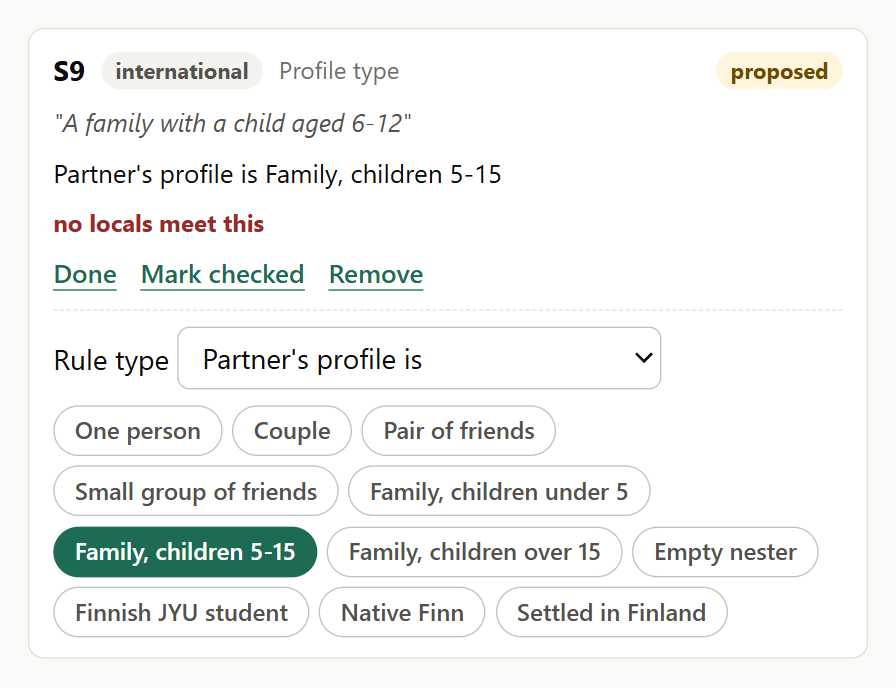
\includegraphics[width=\linewidth]{manual/musthave.png}}
\end{minipage}\hfill
\begin{minipage}[t]{0.49\textwidth}
\vspace{0pt}
Each card shows
\begin{itemize}[leftmargin=*]
  \item who it is and what they chose,
  \item their own words in quotes,
  \item the rule the app will apply,
  \item how many people on the other side meet it.
\end{itemize}
\textcolor{gOne}{\textbf{Red ``no locals meet this''}} means the rule makes a match impossible. Read the
person's words again: is the rule too strict, or does the wish simply not fit this round?

Use \ui{Edit} to change the rule, \ui{Mark checked} when it is right, \ui{Remove} to drop it, and
\ui{Add a must-have} at the bottom for a wish you know about from elsewhere.
\end{minipage}

\begin{tip}
Click the filter \ui{To confirm} and go through the cards one by one. Editing a card marks it as checked.
\end{tip}

\textbf{Staff check.} Some wishes cannot be checked from the survey data, for example an education level or
``not from my own department''. These become a \emph{staff check}: the app does not enforce them, but every
pair that involves this person is marked \flagicon{} so that you can check it by hand.

{\small
\begin{tabularx}{\textwidth}{@{}>{\bfseries}lX@{}}
\toprule
Rule type & What it requires of the partner \\
\midrule
Partner's gender is & a given gender \\
Partner speaks & one of the named languages, at least at the given level \\
A shared language at level & any language both speak, at least at that level \\
Partner has hobby & at least one (or a set number) of the named hobby categories \\
Shared hobby categories & at least this many hobby categories in common \\
Partner's profile is & one of the named profiles (e.g.\ Family, children 5--15) \\
Partner's age within & an age range such as 20--30 \\
Partner's country of origin & one of the named countries \\
Partner has no & a given kind of pet (or no pets at all) \\
Staff check & nothing automatic; you check the pair by hand \\
\bottomrule
\end{tabularx}}

\subsection*{Step 4 \textbullet{} Compute and read the results}
Click \ui{Compute iteration 1} \key{4}. After a few seconds the right side fills.

\textbf{Tiles} \key{B}. \emph{Internationals matched} is the most important number: it is green with \checkmark{}
when everyone has a partner. If not, a red warning \key{C} names each international without a partner
and explains why. \emph{Lowest pair} and \emph{Average pair} show the overall score with its grade.
\emph{Staff checks} and \emph{Gender to resolve} count the pairs you should look at by hand.

\textbf{Grades.} Every score is between 0 and 1 and is turned into a grade:

{\small
\begin{tabularx}{\textwidth}{@{}lllX@{}}
\toprule
Grade & Name & Score & Meaning \\
\midrule
\grade{5} & perfect & 0.90 or more & as good as it gets \\
\grade{4} & very good & 0.80 or more & fully satisfactory \\
\grade{3} & ok / solid & 0.65 or more & a good basis \\
\grade{2} & barely satisfying & 0.50 or more & just acceptable \\
\grade{1} & insufficient & below 0.50 & look closely before confirming \\
\bottomrule
\end{tabularx}}

\textbf{Criteria achievement} \key{D}. One bar per criterion. Each coloured segment counts the pairs with that
grade; point at a segment to see which pairs they are. The number on the right is the average.

\textbf{Constraints in this solution} \key{E}. A tick confirms that a rule is respected in every pair. An
exclamation mark asks you to look, for example at staff checks.

\subsection*{Step 5 \textbullet{} Look at each pair}
Scroll down to \textbf{Pairs}. Each row shows the overall score and the grade of each criterion. Click a row
to open both profiles side by side. Shared hobbies are highlighted, and each must-have shows whether it is met.
A \flagicon{} line quotes a wish to check by hand (Figure~\ref{fig:pairs}).

\begin{figure}[t]
\shot{manual/pairs.png}
\caption{The pairs table with one pair opened: grades per criterion, both profiles, and a wish to check by hand.}
\label{fig:pairs}
\end{figure}

\begin{itemize}[leftmargin=*]
  \item \ui{Lock} keeps a pair you like in the next iteration.
  \item \ui{Forbid} keeps a pair apart in the next iteration, for example after a staff check.
\end{itemize}

\subsection*{Step 6 \textbullet{} Improve: compute again}
Every change on the left (a weight, a must-have, a lock or a forbid) is collected until you click
\ui{Compute iteration 2}, 3, \ldots{} Until then a yellow note says that the results do not include your changes yet.

\textbf{Example.} In the fictional example, iteration~1 matches 19 of 20 internationals. The red warning says
that S9's own must-have rules out all 28 locals: S9 asked for ``a family with a child aged 6--12'', and none of
the locals is such a family. After talking to S9, you change the rule to a \emph{staff check} and compute
again. Iteration~2 matches all 20 (Figure~\ref{fig:iteration2}).

\begin{figure}[t]
\shot{manual/iteration2.png}
\caption{Iteration 2: S9's rule is now a staff check, and all 20 internationals are matched.}
\label{fig:iteration2}
\end{figure}

Each computation adds a chip at the top \key{A}, with the number matched, the lowest grade, the average and how
many pairs changed. Click an older chip to look at it again; \ui{Restore its settings} brings back exactly the
weights, must-haves, locks and forbids of that iteration.

\subsection*{Step 7 \textbullet{} Save}
\begin{tabularx}{\textwidth}{@{}>{\bfseries}l>{\raggedright\arraybackslash}p{4.2cm}X@{}}
\toprule
File & Where & Content \\
\midrule
result.csv & \ui{Save result.csv} \key{F} & one row per pair: scores, grades, locks, notes \\
report.txt & \ui{Save report.txt} \key{F} & summary, grades, pairs, who is not matched and why, review notes, settings \\
settings.csv & Weights: \ui{Save} & the weights and settings, to repeat the run \\
must\_haves.csv & Must-haves: \ui{Save} & the must-haves as you checked them \\
\bottomrule
\end{tabularx}

Your browser puts the files in its Downloads folder. Keep them together with the survey export in a dated folder.
To continue later, load the survey, then \ui{Load} the settings and the must-haves.

\section{How the scores work}
\begin{itemize}[leftmargin=*]
  \item Each criterion gets a score from 0 to 1. \textbf{0.50 means just acceptable, 0.80 fully satisfactory.}
        The defaults: a shared language at \emph{basic} level is just acceptable and \emph{good} is fully
        satisfactory; 2 shared hobby categories are just acceptable and 4 fully satisfactory; an age 25\,\% outside the
        wished range is just acceptable and 10\,\% outside fully satisfactory (inside the range is perfect);
        a missed profile wish counts 25\,\%.
  \item Profile and age are scored from both sides; the pair details show the international's and the local's view.
  \item The overall score \textbf{multiplies} the criteria, with the weights as powers. One weak criterion therefore
        pulls the whole pair down instead of being hidden by an average.
  \item The app first matches \textbf{as many internationals as possible}, then makes the \textbf{lowest pair as good
        as possible}, then the \textbf{total}. Locals may be left without a partner when there are more locals.
  \item \textbf{Blank own gender.} If someone left their own gender empty and the partner wished for a specific
        gender, the pair is shown with a minimum (0, if it does not fit) and a maximum (if it fits). The app uses
        the average and counts the pair under \emph{Gender to resolve}.
\end{itemize}

\section{When something goes wrong}
{\small
\begin{tabularx}{\textwidth}{@{}>{\raggedright\arraybackslash}p{5.4cm}X@{}}
\toprule
Message or problem & What to do \\
\midrule
``This does not look like the survey export'' & Export the survey again as CSV, with both heading rows. \\
``The survey export is missing these questions'' & Export all questions, not a selection. \\
An international is not matched (red warning) & Read the reason. Relax that person's must-have (or make it a staff check),
  remove a lock or forbid, or check the gender and pet answers. Then compute again. \\
``no locals meet this'' on a card & The rule is too strict or misread. Edit it. \\
``Cannot reach the app'' & The app was closed. Start PerfectMatchLFP26.exe again and reload the page. \\
``This session has changed'' & The app was restarted. Reload the page and load the survey again. \\
``The solver could not finish'' & Increase the solver time limit in \ui{Desirability scales and hard rules}. \\
The browser did not open & Open the address shown in your browser, usually http://localhost:8766. \\
Windows blocks the app & The app is not signed. Ask IT to review it. \\
\bottomrule
\end{tabularx}}

\section{Data protection}
\begin{caution}[Personal data]
The survey export, report.txt, result.csv and must\_haves.csv contain participants' IDs and their own words.
Store them like the survey export, in a protected folder, according to the programme's data protection rules,
and delete them when they are no longer needed. Do not send them by e-mail without protection.
\end{caution}
The app runs only on your computer. It does not use the internet, does not store the survey anywhere, and
keeps the data in memory only until you close it. Programme staff review every suggestion before confirming
a pair.

\end{document}
